\section{AnA}

\subsection{Нормальное название}

Synthesis and Biophysical Properties of Arabinonucleic Acids (ANA): Circular
Dichroic Spectra, Melting Temperatures, and Ribonuclease H Susceptibility of
ANA‚RNA Hybrid Duplexes$^\dag$\\
Синтез и биофизичекие свойства арабинуклеиновых кислот: спектр кругового дихроизма, температура плавления, и чувствительность к рибонуклеазе H арабинуклеиновых кислот (ANA), рибонуклеиновых кислот (RNA) гибридных дуплексов
	
	\paragraph{Glossary}
	\begin{itemize}
		\item Circular Dichroic - (Wiki)  is dichroism involving circularly polarized light, i.e., the differential absorption of left- and right-handed light. (короче говоря по разному поглощает свет разной поляризации)
		\item epimer - (Wiki) The two epimers have opposite configuration at only one stereogenic center out of at least two.
		\item antisense agent - (first site in google) Small pieces of DNA or RNA that can bind to specific molecules of RNA. This blocks the ability of the RNA to make a protein or work in other ways. Antisense agents may be used to block the production of proteins needed for cell growth. They are being studied in the treatment of several types of cancer. Also called antisense oligonucleotide.
		\item oligonucleotide - (Wiki) короткий фрагмент ДНК или РНК, получаемый либо путём химического синтеза, либо расщеплением более длинных полинуклеотидов. Используются в качестве зондов или праймеров.
		\item AON - oligonucleotide analogues 
		\item RNase H (abbreviated Ribonuclease H or RNH) is a family of non-sequence-specific endonuclease enzymes that catalyze the cleavage of RNA in an RNA/DNA substrate via a hydrolytic mechanism. 
		\item Escherichia coli - кишечная палочка		
	\end{itemize}
	\subsection{Абстракт}
	Арабинонуклеиновая кислота(АНК), являющаяся 2’-эпимером РНК(потому что около 2’ углерода другое расположение водорода, показано на первой картинке), проявляет хорошие свойства антисмыслового агента, и вот наши догадки почему:
	
	(Вначале определение антисмысловой терапии - это отключение синтеза белков, а для них нужны соответствующие РНК, и уничтожение этих РНК замедлит/отключит синтез белков)
	
	Рибонуклеаза(далее - РНаза) уничтожает РНК, если РНК закреплена на комплементарной ДНК. Дуплекс комплементарных АНК и РНК очень похож по структуре на комплекс комплементарных ДНК и РНК, что, вероятно, и провоцирует активность РНазы. Помимо другого расположения атомов около 2’-углерода, скорее всего наблюдается еще и некоторая деформация сахарного кольца, которое больше похоже на таковое у ДНК, чем у РНК.
	Поэтому спектр дуплексов АНК/РНК очень похож на соответствующий спектр дуплексов АНК/РНК. Также, ОН группа около 2’-углерода в дуплексе с РНК направлена в большую бороздку дуплекса(картинка в конце статьи) и не мешает активности РНазы.
	Эти вещи позволяют сделать вывод, что они - ключевые в активации РНазы.
	
	\subsection{Картинки}
	\begin{figure}[H]
		\centering
		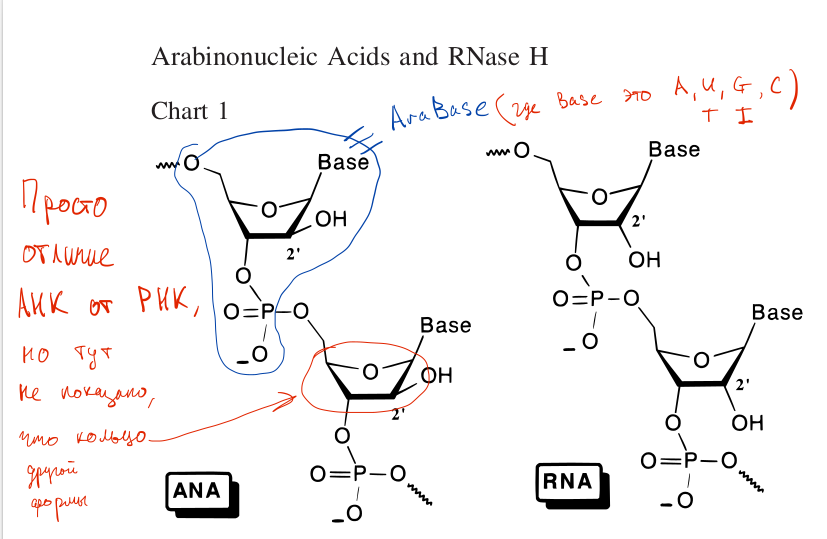
\includegraphics[scale = 0.3]{4_1}
	\end{figure}
\begin{figure}[H]
	\centering
	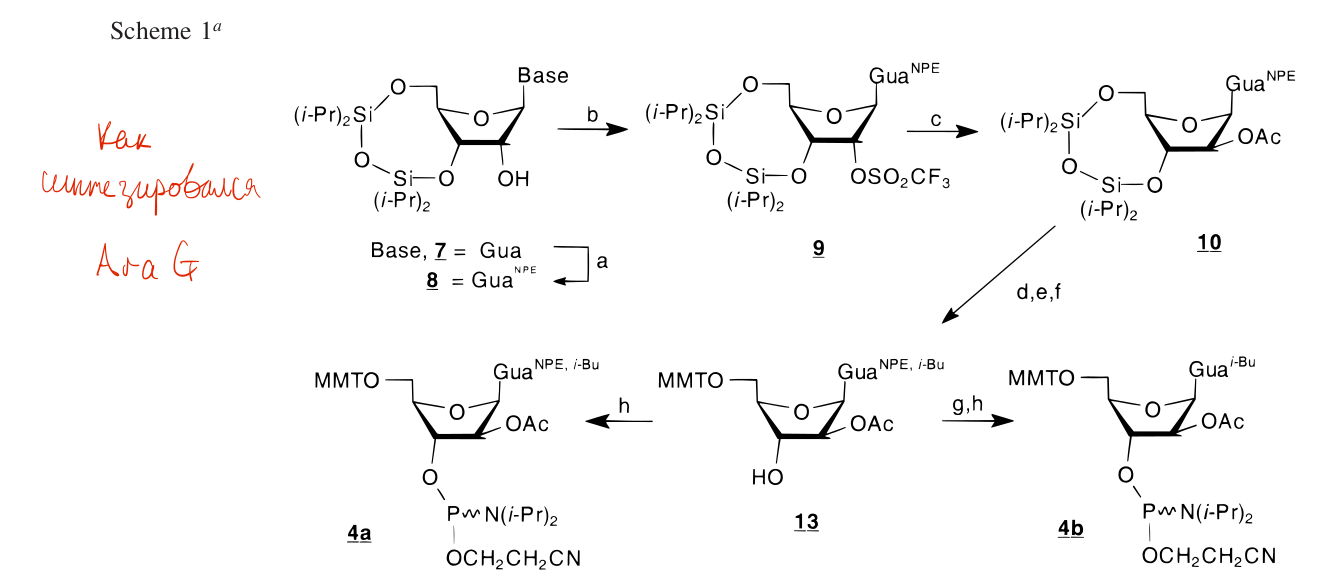
\includegraphics[scale = 0.3]{Pictures/4_2}
\end{figure}
	\begin{figure}[H]
		\centering
		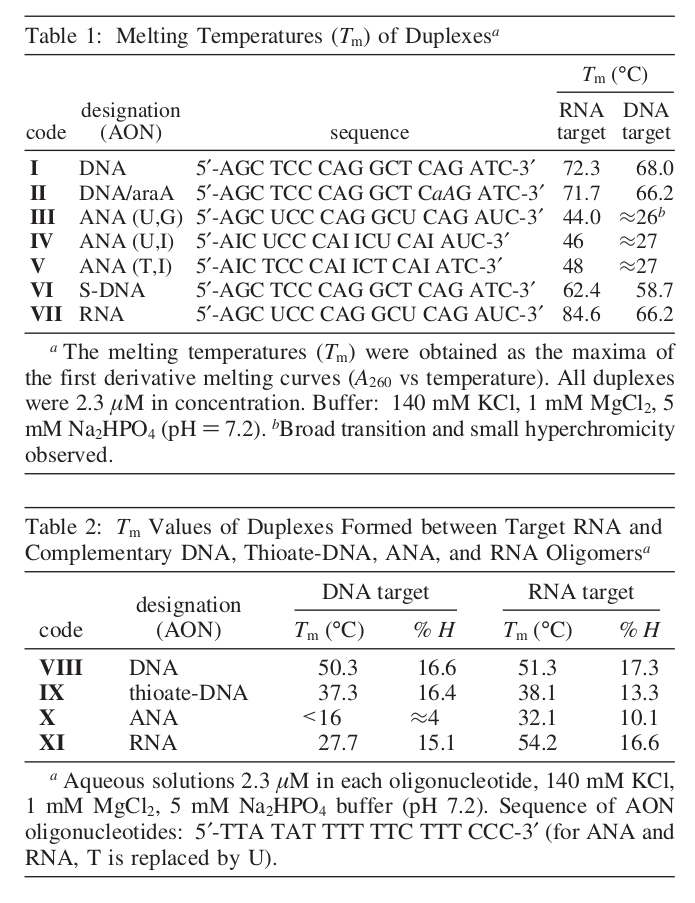
\includegraphics[scale = 0.3]{Pictures/4_3}
		\caption{Табличка с цепочками нуклеиновых кислот, были синтезированы короткие цепочки, указаны блоки с основаниями. aA в цепочке второй ДНК значит,  то один из блоков в цепочке заменен на арабинонуклеиновый аналог.
			Указаны температуры плавления для дуплексов соответствующей нуклеиновой кислоты с комплементарной РНК и ДНК(предпоследний и последний столбцы). Плавлением считается момент, когда дуплекс распадается обратно на 2 цепочки.}
	\end{figure}
	\begin{figure}[H]
		\centering
		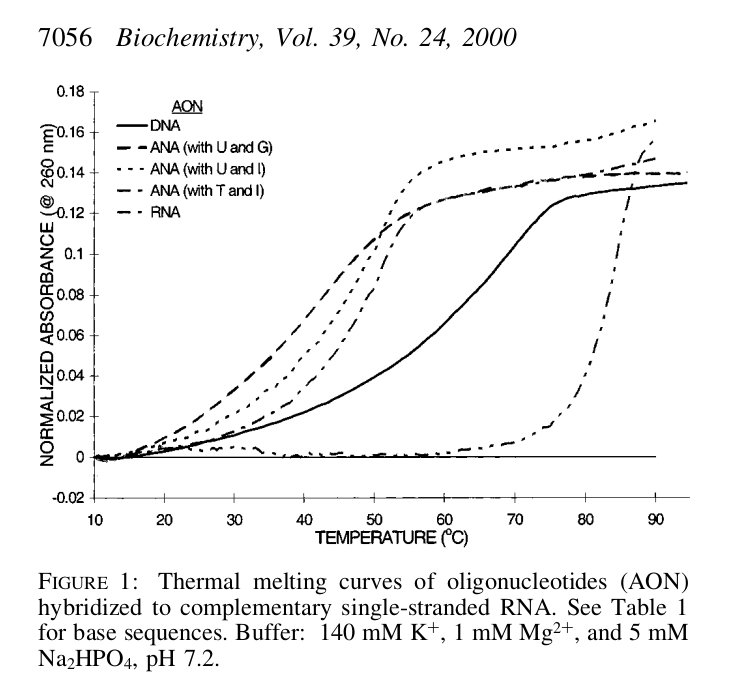
\includegraphics[scale = 0.3]{Pictures/4_4}
		\caption{График плавления нуклеиновой кислоты(указаны слева) в дуплексе с РНК. Поглощение указанной длины волны соответствует тому, что в растворе распались дуплексы и отдельные цепочки начали поглощать.}
	\end{figure}
	\begin{figure}[H]
		\centering
		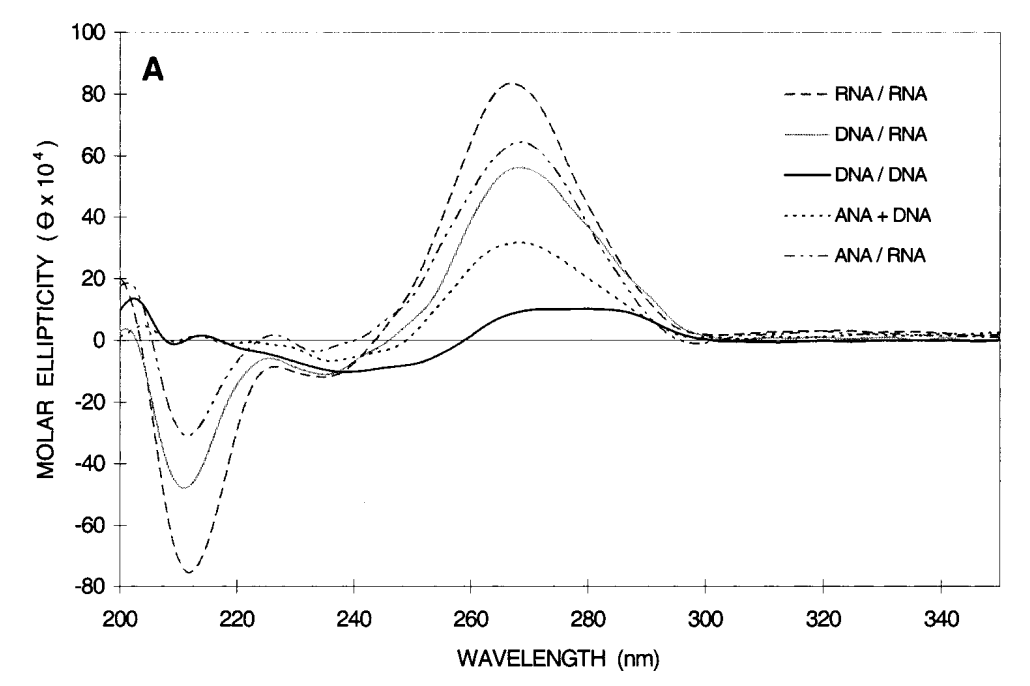
\includegraphics[scale = 0.3]{Pictures/4_5}
		\caption{Спектры кругового дихроизма соответствующих дуплексов(АНК и ДНК не соединяются в дуплекс)
			Видно, что АНК/РНК очень похоже на ДНК/РНК}
	\end{figure}
	\begin{figure}[H]
		\centering
		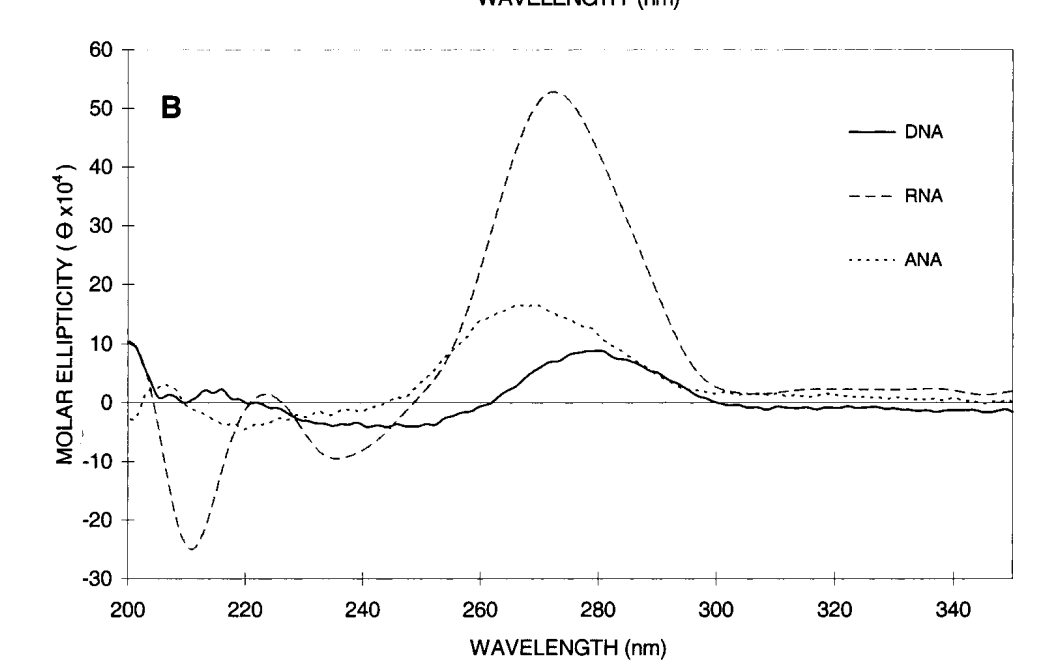
\includegraphics[scale = 0.3]{Pictures/4_6}
		\caption{Аналогично, но КД спектр уже просто для цепочек.
			Видно большую схожесть АНК с ДНК}
	\end{figure}
	\begin{figure}[H]
		\centering
		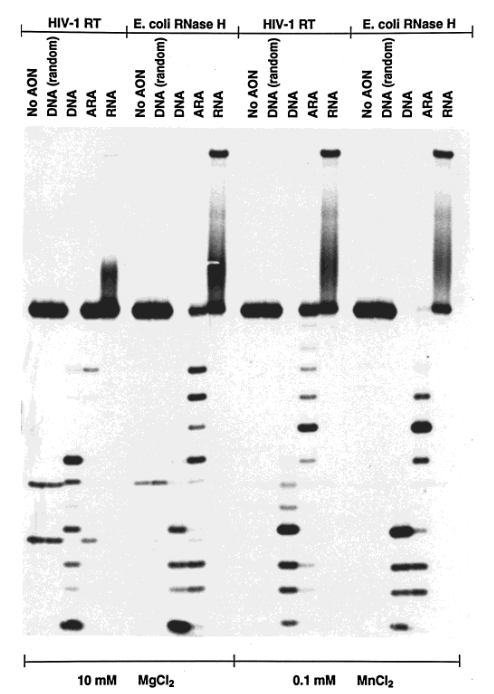
\includegraphics[scale = 0.3]{Pictures/4_7}
		\caption{Гидролиз в геле, куда с РНК смешивается указанная нуклеиновая кислота, и если РНаза проявляет активность, то появляются маленькие кусочки разрезанной РНК и они спускаются ниже, чем длинные исходные цепочки}
	\end{figure}
	\begin{figure}[H]
		\centering
		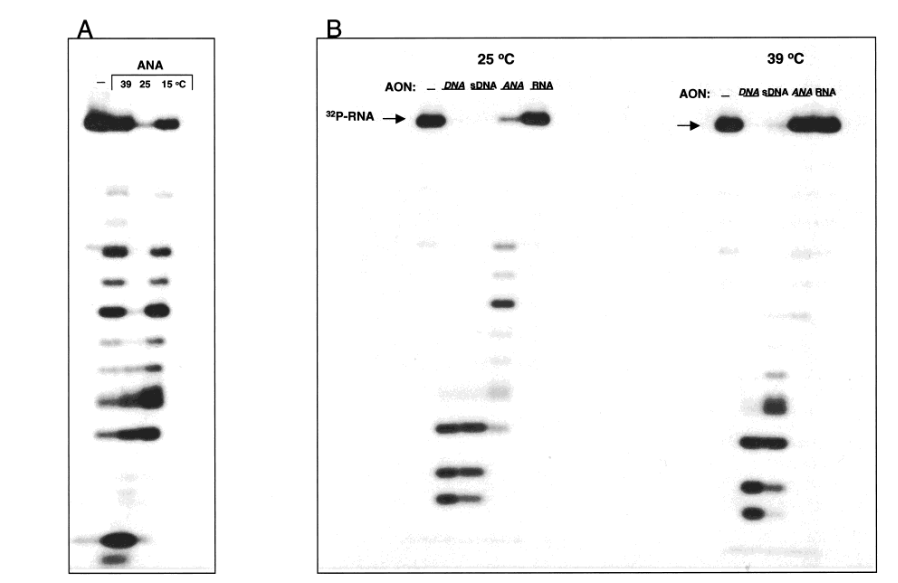
\includegraphics[scale = 0.3]{Pictures/4_8}
		Как и предыдущая картинка, но тут исследуется зависимость от температуры и другая цепочка АНК в картинке В.
		Видно, что при большой температуре АНК уже плохо работает(связано с тем, что дуплексы уже близки к температурам плавления)
	\end{figure}
	\begin{figure}[H]
		\centering
		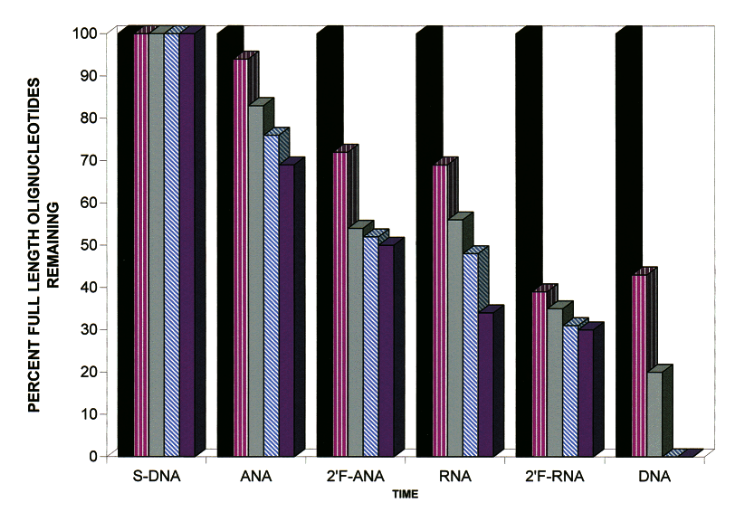
\includegraphics[scale = 0.3]{Pictures/4_9}
		\caption{snake venom phosphodiesterase (SVPDE) — это штука, которая разрушает нуклеиновую кислоту, и исследуется устойчивость нуклеиновый кислот с течением времени в присутствии это фосфодиэстеразы.}
	\end{figure}
	\begin{figure}[H]
		\centering
		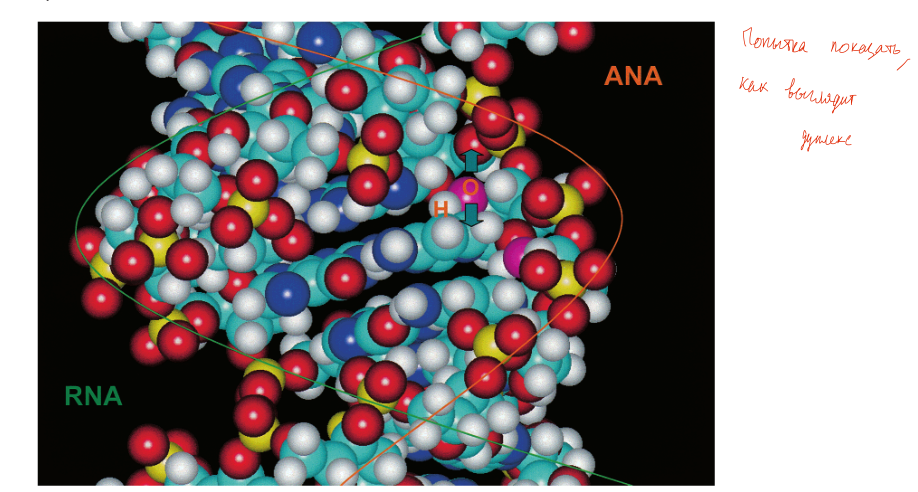
\includegraphics[scale = 0.4]{Pictures/4_10}
		
	\end{figure}
	\begin{figure}[H]
		\centering
		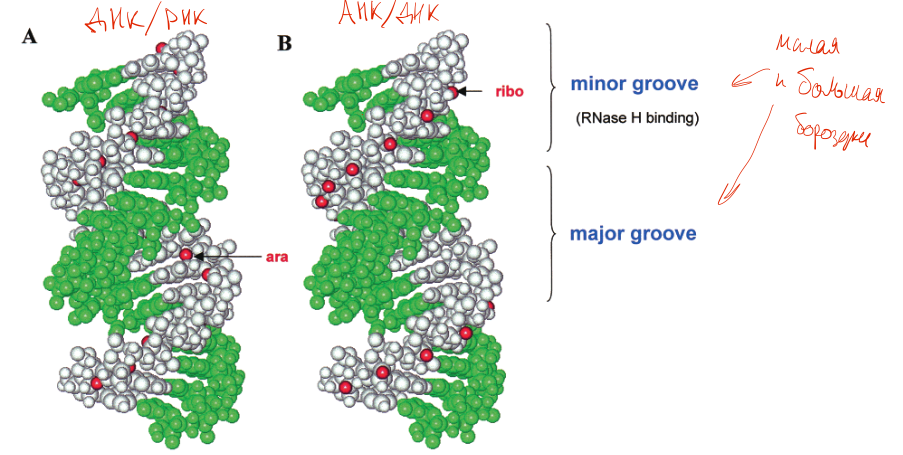
\includegraphics[scale = 0.4]{Pictures/4_11}
		\caption{На рисунке изображены дуплексы ДНК/РНК, но на А показана арабино конфигурация 2’H атома, а на рисунке B - рибо конфигурация 2’’H атома.
			Так как рибонуклеаза распознаёт дуплекс по его малой бороздке, а также видно, что арабино конфигурация мало влияет на конфигурацию этой малой бороздки, то АНК/РНК хорошо походит на истинный дуплекс ДНК/РНК. В рибо конфигурации же, наоборот - из малой бороздки «видно» мешающую гидроксильную группу, торчащую наружу.}
	\end{figure}
	